\documentclass[a4paper]{article}
\usepackage{listings}
\usepackage{vntex}
%\usepackage[english,vietnam]{babel}
%\usepackage[utf8]{inputenc}

%\usepackage[utf8]{inputenc}
%\usepackage[francais]{babel}
\usepackage{a4wide,amssymb,epsfig,latexsym,array,hhline,fancyhdr}

\usepackage{amsmath}
\usepackage{amsthm}
\usepackage{multicol,longtable,amscd}
\usepackage{diagbox}%Make diagonal lines in tables
\usepackage{booktabs}
\usepackage{alltt}
\usepackage[framemethod=tikz]{mdframed}% For highlighting paragraph backgrounds
\usepackage{caption,subcaption}

\usepackage{lastpage}
\usepackage[lined,boxed,commentsnumbered]{algorithm2e}
\usepackage{enumerate}
\usepackage{color}
\definecolor{mygreen}{RGB}{28,172,0} % color values Red, Green, Blue
\definecolor{mylilas}{RGB}{170,55,241}
\usepackage{graphicx}							% Standard graphics package
\usepackage{array}
\usepackage{tabularx, caption}
\usepackage{multirow}
\usepackage{multicol}
\usepackage{rotating}
\usepackage{graphics}
\usepackage{geometry}
\usepackage{setspace}
\usepackage{epsfig}
\usepackage{tikz}
\usetikzlibrary{arrows,snakes,backgrounds}
\usepackage[unicode]{hyperref}
\hypersetup{urlcolor=blue,linkcolor=black,citecolor=black,colorlinks=true} 
%\usepackage{pstcol} 								% PSTricks with the standard color package

\newtheorem{theorem}{{\bf Định lý}}
\newtheorem{property}{{\bf Tính chất}}
\newtheorem{proposition}{{\bf Mệnh đề}}
\newtheorem{corollary}[proposition]{{\bf Hệ quả}}
\newtheorem{lemma}[proposition]{{\bf Bổ đề}}


%\usepackage{fancyhdr}
\setlength{\headheight}{40pt}
\pagestyle{fancy}
\fancyhead{} % clear all header fields
\fancyhead[L]{
 \begin{tabular}{rl}
    \begin{picture}(25,15)(0,0)
    \put(0,-8){
\includegraphics[width=8mm, height=8mm]{Images/hcmut.png}}
    %\put(0,-8){\epsfig{width=10mm,figure=hcmut.eps}}
   \end{picture}&
	%
\includegraphics[width=8mm, height=8mm]{hcmut.png} & %
	\begin{tabular}{l}
		\textbf{\bf \ttfamily Trường Đại Học Bách Khoa Tp.Hồ Chí Minh}\\
		\textbf{\bf \ttfamily Khoa Khoa Học và Kỹ Thuật Máy Tính}
	\end{tabular} 	
 \end{tabular}
}
\fancyhead[R]{
	\begin{tabular}{l}
		\tiny \bf \\
		\tiny \bf 
	\end{tabular}  }
\fancyfoot{} % clear all footer fields
\fancyfoot[L]{\scriptsize \ttfamily Bài tập lớn môn Mô hình hóa toán học (CO2011) - Niên khóa 2019-2020}
\fancyfoot[R]{\scriptsize \ttfamily Trang {\thepage}/\pageref{LastPage}}
\renewcommand{\headrulewidth}{0.3pt}
\renewcommand{\footrulewidth}{0.3pt}


%%%
\setcounter{secnumdepth}{4}
\setcounter{tocdepth}{3}
\makeatletter
\newcounter {subsubsubsection}[subsubsection]
\renewcommand\thesubsubsubsection{\thesubsubsection .\@alph\c@subsubsubsection}
\newcommand\subsubsubsection{\@startsection{subsubsubsection}{4}{\z@}%
                                     {-3.25ex\@plus -1ex \@minus -.2ex}%
                                     {1.5ex \@plus .2ex}%
                                     {\normalfont\normalsize\bfseries}}
\newcommand*\l@subsubsubsection{\@dottedtocline{3}{10.0em}{4.1em}}
\newcommand*{\subsubsubsectionmark}[1]{}
\makeatother

\everymath{\color{blue}}%make in-line maths symbols blue to read/check easily

\sloppy
\captionsetup[figure]{labelfont={small,bf},textfont={small,it},belowskip=-1pt,aboveskip=-9pt}
%space remove between caption, figure, and text
\captionsetup[table]{labelfont={small,bf},textfont={small,it},belowskip=-1pt,aboveskip=7pt}
%space remove between caption, table, and text

%\floatplacement{figure}{H}%forced here float placement automatically for figures
%\floatplacement{table}{H}%forced here float placement automatically for table
%the following settings (11 lines) are to remove white space before or after the figures and tables
%\setcounter{topnumber}{2}
%\setcounter{bottomnumber}{2}
%\setcounter{totalnumber}{4}
%\renewcommand{\topfraction}{0.85}
%\renewcommand{\bottomfraction}{0.85}
%\renewcommand{\textfraction}{0.15}
%\renewcommand{\floatpagefraction}{0.8}
%\renewcommand{\textfraction}{0.1}
\setlength{\floatsep}{5pt plus 2pt minus 2pt}
\setlength{\textfloatsep}{5pt plus 2pt minus 2pt}
\setlength{\intextsep}{10pt plus 2pt minus 2pt}

% Typesetting Listings
\usepackage{xcolor}
\usepackage{color}
\definecolor{listinggray}{gray}{0.9}
\definecolor{lbcolor}{rgb}{0.9,0.9,0.9}
\definecolor{Darkgreen}{rgb}{0.1,0.6,0.1}
\definecolor{whitesmoke}{rgb}{0.99, 0.99,0.99}

\lstset{language=Matlab,%
    %basicstyle=\color{red},
    breaklines=true,%
    morekeywords={matlab2tikz},
    keywordstyle=\color{blue},%
    morekeywords=[2]{1}, keywordstyle=[2]{\color{black}},
    identifierstyle=\color{black},%
    stringstyle=\color{mylilas},
    commentstyle=\color{mygreen},%
    showstringspaces=false,%without this there will be a symbol in the places where there is a space
    numbers=left,%
    numberstyle={\tiny \color{black}},% size of the numbers
    numbersep=9pt, % this defines how far the numbers are from the text
    emph=[1]{for,end,break},emphstyle=[1]\color{red}, %some words to emphasise
    %emph=[2]{word1,word2}, emphstyle=[2]{style},    
}

\begin{document}
\begin{titlepage}
\begin{center}
ĐẠI HỌC QUỐC GIA THÀNH PHỐ HỒ CHÍ MINH \\
TRƯỜNG ĐẠI HỌC BÁCH KHOA \\
KHOA KHOA HỌC - KỸ THUẬT MÁY TÍNH 
\end{center}

\vspace{1cm}

\begin{figure}[h!]
\begin{center}

\includegraphics[width=3cm]{Images/hcmut.png}
\end{center}
\end{figure}

\vspace{1cm}


\begin{center}
\begin{tabular}{c}
\multicolumn{1}{l}{\textbf{{\Large MÔ HÌNH HÓA TOÁN HỌC (CO2011)}}}\\
~~\\
\hline
\\
\multicolumn{1}{l}{\textbf{{\Large Nhóm: TTSL - Bài tập lớn}}}\\
\\
\textbf{{\Huge Mô hình SIR}} \\
\textbf{{\Huge trong dự báo COVID-19}}\\
\\
\hline
\end{tabular}
\end{center}

\vspace{1.5cm}

\begin{table}[h]
\begin{tabular}{rrl}
\hspace{5 cm} & GVHD: & Nguyễn An Khương\\
\hspace{5 cm} &  & Nguyễn TIến Thịnh\\

& SV thực hiện: & Nguyễn Văn A -- 22102134 \\
& & Trần Văn B -- 88471475 \\
& & Lê Thị C -- 36811334 \\
& & Phạm Ngọc D -- 97501334 \\
& & Kiều Thị E -- 12341334 \\
\end{tabular}
\end{table}
\vspace{1.5cm}
\begin{center}
{\footnotesize Tp. Hồ Chí Minh, Tháng .../2020}
\end{center}
\end{titlepage}

% Table of contents
\newpage
\tableofcontents

\newpage
\section{Bài toán 1}

\newpage
\section{Bài toán 2}
\subsection{Cơ sở lý thuyết}
Với một số gia $h$ đủ nhỏ, đạo hàm của một hàm số tại một điểm $x_0$ bất kỳ có thể coi như tương đương với:
\[f'(x_0) \approx \frac{f(x_0+h)-f(x_0)}{h}\]
Về hình học, coi như cát tuyến đi qua 2 điểm $(x_0, f(x_0))$ và $(x_0+h, f(x_0+h))$ là tiếp tuyến tại $x_0$ khi khoảng cách $h$ không đáng kể.Tương đương:
\[ f(x_0+h) \approx f(x_0) + h*f'(x_0) \]
Một phương trình vi phân bậc nhất có dạng:
\[  f'(x) = g(x,f(x))  \]
Như vậy với $x_0$ bất kỳ, ta luôn xấp xỉ được giá trị hàm tại $x=x_0+h$ bằng công thức:
\[ f(x_0+h) \approx f(x_0) + h*g(x_0,f(x_0)) \]
Nếu ta tách toàn bộ miền xác định của $x$ thành các đoạn có độ dài là $h$, miền giá trị $y$ cũng có thể được xấp xỉ bằng dãy ${y_n}$ với mỗi giá trị $y_n$ được tính bằng:
\[ y_n \approx y_{n-1} + h*g(x_{n-1},y_{n-1}) \]
với bước xấp xỉ $h = x_n - x_{n-1}$ đủ nhỏ và $g(x_{n-1},y_{n-1})$ được gọi là độ dốc của đường cong $f(x)$ tại $x_0$. Tương tự đối với hệ phương trình vi phân bậc nhất, với $Y(x) = (y_1(x), y_2(x),... , y_n(x))^T$ ta có:
\[ Y_n \approx Y_{n-1} + h*G(x_{n-1},Y_{n-1}) \]
Dựa theo công thức này, nếu biết $x_0$ và $Y_0$, ta có thể xấp xỉ được nghiệm $Y(x)$. Trong bài toán SIR, nếu biết được toàn bộ các thông số tại thời điểm bắt đầu khảo sát, với bước xấp xỉ đủ nhỏ ta có thể tính xấp xỉ được hệ nghiệm.
\subsection{Code}\label{Code-Euler}
\begin{itemize}
\item Nhóm sử dụng công cụ lập trình và hổ trợ tính toán Matlab cho phần hiện thực.
\item Với phương pháp Euler thì trong chương trình, nhóm chọn step size ($ \Delta t $) = 0.1. 
\item Đoạn chương trình như sau:
\lstinputlisting{Code/baitoan2/SIR_Euler.m}
\end{itemize}
\subsection{Ví dụ}
Giả sử rằng có một loại cúm đang lây lan trong cộng đồng dân cư và có những điều kiện ràng buộc sau:
	\begin{itemize}
		\item Cộng đồng này đang bị cách li, không ai được ra và cũng không ai được vào
		\item Một người khi mắc bệnh và hồi phục thì không còn mắc bệnh này lần nữa
		\item Tạị thời điểm bắt đầu khảo sát $t0$ thì số người có khả năng mắc bệnh, nhiễm bệnh và hồi phục lần lượt là 950, 50 và 0 người.
	 \end{itemize}
Trong phần này, nhóm sẽ sử dụng cộng đồng dân cư trên để lấy 2 ví dụ về việc sử dụng phương pháp Euler tìm nghiệm cho hệ SIR. Với 2 ví dụ này thì hệ SIR chỉ khác nhau ở 2 hệ số $ \beta $ và $ \gamma $
\subsubsection{Ví dụ 1}\label{vd1-ppEuler}
\begin{enumerate}[a)]
\item \textbf{Điều kiện đầu}
	\begin{itemize}
		\item Hệ số tiếp xúc $ \beta $ = 0.4
		\item Hệ số phục hồi $ \gamma $ = 0.5
		\item Biến thời gian $ t $ = 12
		\item $ S(t0) $ = 950 , $ I(t0) $ = 50, $ R(t0) $ = 0
	\end{itemize}

\item \textbf {Hệ SIR thành lập được}
	\begin{align} \label{hptEuler1} \tag{I}
	    \begin{split} 
	        &\frac{dS}{dt} = -0.0004IS \\
	        &\frac{dI}{dt} = 0.0004IS - 0.5I \\
	        &\frac{dR}{dt} = 0.5I
	    \end{split}
	\end{align}
\item \textbf{Dùng chương trình đã viết ở  phần \ref{Code-Euler} tìm nghiệm hệ phương trình \eqref{hptEuler1} }\\
	\\Trong commandline Matlab, ta dùng lệnh sau để tìm nghiệm của hệ
	\begin{mdframed}[hidealllines=true,backgroundcolor=magenta!10]
	\begin{alltt}
	\textit{
	>> Output = SIR_Euler(12,0.4,0.5,950,50,0)
	}
	\end{alltt}
	\end{mdframed}
	
	\textbf{Kết quả:}\\
	Sau khi chạy lệnh trên ta được kết quả như sau
	\begin{mdframed}[hidealllines=true,backgroundcolor=blue!10]
	\begin{alltt}
	\textit{
	 Output = 844.4828    8.4349  147.0823
	}
	\end{alltt}
	\end{mdframed}
	Vậy tại thời điểm $ t = 12 $ thì:
	\begin{itemize}
		\item Số người có nguy cơ nhiễm bệnh là khoảng 845 người
		\item Số người nhiễm bệnh là khoảng 8 người
		\item Số người hồi phục là khoảng 147 người
	\end{itemize}

\item \textbf{Đồ thị biểu diễn nghiệm xấp xỉ - Hình~\ref{Fig:vd1}}.
	\begin{figure}[h!]
		\begin{center}
		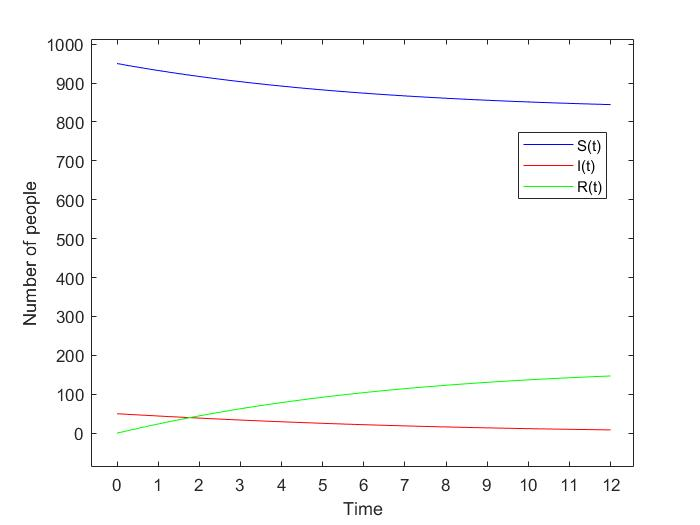
\includegraphics[scale=0.5]{Images/baitoan2/p1.jpg}
		\end{center}
		\caption{Đồ thị biểu diễn nghiệm xấp xỉ \nameref{vd1-ppEuler}}\label{Fig:vd1}
	\end{figure}
	
\item \textbf{Nhận xét}
	\begin{itemize}
		\item Số người nhiễm bệnh tại từng thời điểm sẽ giảm dần
		\item Tại thời điểm $ t = 12 $ thì số người có nguy cơ nhiễm bệnh còn khoảng 845 người, nghĩa là có thêm khoảng 105 (được tính bằng $ S(t)-S(t0) $) người chuyển từ nhóm có nguy cơ sang nhóm nhiễm bệnh, chiếm tỉ lệ nhỏ so với số người có nguy cơ ban đầu. Điều này chứng tỏ dịch bệnh đã không bùng phát.
		\item Như vậy, ta thấy với  tỉ số $ \frac{\beta}{\gamma} = \frac{0.4}{0.5} = 0.8 <1$  thì dịch bệnh sẽ không có nguy cơ bùng phát. 
	\end{itemize}
\end{enumerate}

\subsubsection{Ví dụ 2}\label{vd2-ppEuler}
\begin{enumerate}[a)]
\item \textbf{Điều kiện đầu}
	\begin{itemize}
		\item Hệ số lây nhiễm $ \beta $ = 2
		\item Hệ số phục hồi $ \gamma $ = 0.5
		\item Biến thời gian $ t $ = 12
		\item $ S(t0) $ = 950 , $ I(t0) $ = 50, $ R(t0) $ = 0
	\end{itemize}

\item \textbf {Hệ SIR thành lập được}
	\begin{align} \label{hptEuler2} \tag{II}
	    \begin{split} 
	        &\frac{dS}{dt} = -0.002IS \\
	        &\frac{dI}{dt} = 0.002IS - 0.5I \\
	        &\frac{dR}{dt} = 0.5I
	    \end{split}
	\end{align}
\item \textbf{Dùng chương trình đã viết ở phần \ref{Code-Euler} tìm nghiệm hệ phương trình \eqref{hptEuler2} }\\
	\\Trong commandline Matlab, ta dùng lệnh sau để tìm nghiệm của hệ
	\begin{mdframed}[hidealllines=true,backgroundcolor=magenta!10]
	\begin{alltt}
	\textit{
	>> Output = SIR_Euler(12,2,0.5,950,50,0)
	}
	\end{alltt}
	\end{mdframed}
	
	\textbf{Kết quả:}\\
	Sau khi chạy lệnh trên ta được kết quả như sau
	\begin{mdframed}[hidealllines=true,backgroundcolor=blue!10]
	\begin{alltt}
	\textit{
	 Output = 17.2474    9.1779  973.5747
	}
	\end{alltt}
	\end{mdframed}
	Vậy tại thời điểm $ t = 12 $ thì:
	\begin{itemize}
		\item Số người có nguy cơ nhiễm bệnh là khoảng 17 người
		\item Số người nhiễm bệnh là khoảng 9 người
		\item Số người hồi phục là khoảng 974 người
	\end{itemize}

\item \textbf{Đồ thị biểu diễn nghiệm xấp xỉ - Hình~\ref{Fig:vd2}}.
	\begin{figure}[h!]
		\begin{center}
		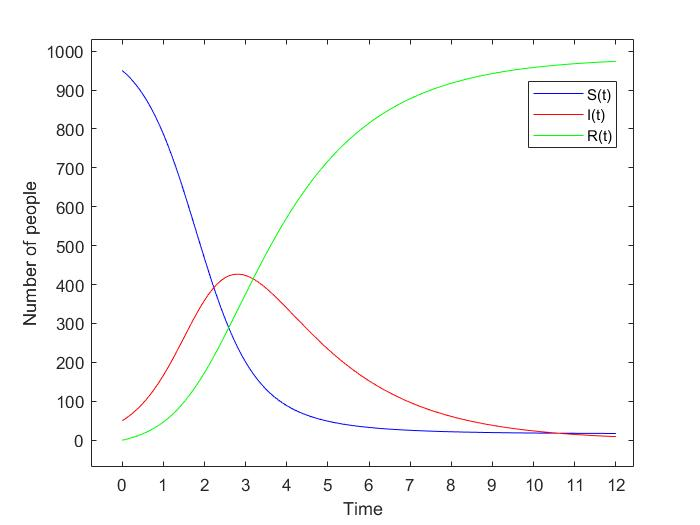
\includegraphics[scale=0.5]{Images/baitoan2/p2.jpg}
		\end{center}
		\caption{Đồ thị biểu diễn nghiệm xấp xỉ \nameref{vd2-ppEuler}}\label{Fig:vd2}
	\end{figure}
	
\item \textbf{Nhận xét}
	\begin{itemize}
		\item Số người nhiễm bệnh tại từng thời điểm sẽ tăng trong khoảng thời gian từ 0 đến 3 và sau đó giảm dần. Tại thời điểm t=3 thì số người trong nhóm nhiễm bệnh lên đến 400 người.
		\item Tại thời điểm $ t = 12 $ thì số người có nguy cơ nhiễm bệnh còn khoảng 17 người, nghĩa là có thêm khoảng 933 (được tính bằng $ S(t)-S(t0) $) người chuyển từ nhóm có nguy cơ sang nhóm nhiễm bệnh, chiếm tỉ lệ cao so với số người có nguy cơ ban đầu. Điều này chứng tỏ dịch bệnh đã bùng phát mạnh mẽ, gần như cả cộng đồng đều đã nhiễm bệnh.
		\item Như vậy, ta thấy với  tỉ số $ \frac{\beta}{\gamma} = \frac{2}{0.5} = 4 > 1$ thì dịch bệnh sẽ  bùng phát. 
	\end{itemize}
\end{enumerate}

\subsection{Kết luận}
Như vậy trong phần này, nhóm đã trình bày về phương pháp Euler trong việc tìm nghiệm cho hệ SIR. Nhóm đã trình bày phần chương trình (code dược viết bằng Matlab) cũng như đưa ra một số ví dụ kiểm tra và sử dụng chương trình. Thông qua các ví dụ thì chúng ta đã phần nào hình dung được tỉ lệ $ \frac{\beta}{\gamma} $ ảnh hưởng như thế nào đến dịch bệnh. Trong phần tiếp theo nhóm sẽ làm rõ hơn những vấn đề liên quan đến tỉ lệ này

\newpage
\section{Bài toán 3}
\end{document}